\documentclass[10pt,compress,serif,aspectratio=169]{beamer}
\usepackage{pres2023_169}
\usepackage[utf8]{inputenc}
\usepackage{fourier}

\newcommand{\todo}[1]{{\color{red} TODO: #1}}
\graphicspath{{figures/}}
 
\begin{document}

\begin{frame}[t]
  \begin{center}
  \vspace{1cm}
  {An Open Source Project for Dissemination of Computational
Solid Mechanics (DCSM)}\\
  \vspace{.5cm}
  {\Large Guillaume Anciaux}\\{LSMS, IIC, ENAC, EPFL}\\
  \end{center}
\vspace{.5cm}
\fig{.13}{2560px-Logo_EPFL.svg.png}\qquad \fig{.18}{ethr_en_rgb_black.pdf} \\ \vspace{.2cm}
\fig{.22}{logo2023.pdf} \qquad \fig{.15}{episciences-logo}\\\fig{.18}{solidipes}\\{\small\url{https://gitlab.com/dcsm/solidipes}}\\
\end{frame}

%%%

% \begin{frame}[t]{Outlook}
% \begin{columns}[t]
%         \begin{column}{.5\textwidth}
%             \tableofcontents[sections={1-3}]
%         \end{column}
%         \begin{column}{.5\textwidth}
%             \tableofcontents[sections={4-7}]
%         \end{column}
%     \end{columns}
% \end{frame}


%%%

\section{motivation}
\subsection{unwanted situations}
\begin{frame}{Did it ever happen to you ?}
\fig{1}{notfound-dataset.pdf}
\end{frame}


%%%

\subsection{Publishing datasets}
\begin{frame}{Publishing datasets: Where?}
\textbf{\href{https://zenodo.org/}{Zenodo}}
\begin{itemize}
  \item Long term preservation $\Rightarrow$ \href{https://about.zenodo.org/policies/}{for 20 more years from now}
  \item Generalist $\Rightarrow$ stores anything, no checks
  \item $<$ 50 GB limit 
  \item Read-only datasets after publication
  \item Modifiable metadata 
\pause
\item \textbf{What content ? Who checks ?}
\begin{itemize}
  \item[-] At the moment \textbf{no one but the owner} (Can publish anything)
  \item[+] Curation perspective (e.g. \href{https://about.zenodo.org/projects/horizon-zen/}{Horizon-Zen project}) 
 \end{itemize}
\pause
\end{itemize}
\vfill
\textbf{Institutional/focused repositories ?}

\begin{columns}[t]
        \begin{column}{.5\textwidth}
\begin{itemize}
  \item \href{https://www.materialscloud.org/home}{Material's Cloud} with \href{https://www.aiida.net/}{Aiida}

  \item \href{https://www.research-collection.ethz.ch/}{Research collection at ETHz}
\end{itemize}
        \end{column}
        \begin{column}{.5\textwidth}
\begin{itemize}
  \item \href{https://livmats-data.vm.uni-freiburg.de/}{LivMatS} with \href{https://github.com/jic-dtool/dtool}{dtool}
  \item \href{https://dataverse.org/installations}{Dataverse} 
\end{itemize}
        \end{column}
    \end{columns}

\vfill

\begin{center}
many others.... \pause \alert{all needing curation}
\end{center}
\end{frame}

%%%

%\subsection{unwanted situations}
%\begin{frame}{Did it ever happen to you ?}
%
%  \begin{itemize}
%    \item fail compiling a (old) published code
%   \item re-run leads to different results, or fails
%    \item horror times in assembling dataset for AI
%\end{itemize}
%\fig{.4}{compilation-error}
%\end{frame}


%%%

\subsection{Definition curation}
\begin{frame}{Definitions: \href{https://zenodo.org/records/10626170}{CODATA RDM Terminology}}

\textit{\textbf{Data Curation} ensures usefulness for discovery and reuse.}\\
\begin{quote} 
\begin{itemize}
  \item validation of the data (encoding, file formats)
  \item description completeness (documentation, annotation)
  \item discipline dependent (question of vocabulary, formats, )
\end{itemize}
  \end{quote}

\pause
\vfill

Who does it ?
\begin{itemize}
  \item journals
  \item universities (arXiv, HAL)
  \item specialized archivists (e.g. astronomy with NASA, ESA, neurologists and brain MRI)
\end{itemize}
\pause
\vfill

\begin{center}
  \alert{{\Large\textbf{Data curation}} is a central pillar in fostering scientific discoveries}\\
\vfill
\pause
 \alert{Sometimes difficult to {\Large\textbf{convince}} researchers to cure data}\\
\vfill
\pause
  \alert{My personal belief is that {\Large \textbf{journals}} should play a role}

\end{center}
\end{frame}



%%% 

%\subsection{The problem: not easy to convince people to do the work}
%\begin{frame}{Difficulty: Convincing researchers}
%  \fig{.48}{comics1}
%  \fig{.35}{comics2}
%\begin{center}
%  \url{https://zenodo.org/records/10108736}
%  \end{center}
%\vfill
%\begin{center}
%\pause
%    {\alert{\Large My personal belief is that journals should play a role}}
%\end{center}
%\end{frame}

%%%

\section{JTCAM presentation}
\subsection{JTCAM presentation}
\begin{frame}[t]{}

\fig{.6}{logo2023}\newline

  \begin{quote}
    is a {\huge \textbf{Diamond open access}} journal, i.e. published with \textbf{no fees to either reader or author.} \newline
\end{quote}

  \begin{quote}
      and is an {\huge \textbf{overlay}} journal, i.e. that does not produce its own content, but selects from texts that are \textbf{already freely available online} (thanks to \href{https://www.episciences.org/}{Episciences!}).
\newline
\end{quote}

 \begin{itemize}
 \item Editorial process entirely controlled by researchers   
 \item Wide spectrum: theoretical, applied, numerical, experimental
\pause
 \item Recent attempt to include \textbf{Data curation} in the publication process 

 \end{itemize}
\end{frame}

%%%%
\subsection{JTCAM Publication process}
\begin{frame}[t]{JTCAM: publication process}
 \begin{center}%
   \only<1>{\fig{1}{epirevue_0d}}%
   \only<2>{\fig{1}{epirevue_1d}}%
   \only<3>{\fig{1}{epirevue_2d}}%
    \only<4>{\fig{1}{epirevue_3d}}%
   \only<5>{\fig{1}{epirevue_4d}}%
   \only<6>{\fig{1}{epirevue_5d}}%
 \end{center}%
\end{frame}

%%%% 

\subsection{JTCAM dataset curation policy }
\begin{frame}{JTCAM dataset curation policy => FAIR}

The following criteria are required in order to accept a submission to the JTCAM community:

\begin{itemize}
\item Must be Open Access
\item Ownership described in depth
\item Detailed description (using standard ontologies or controlled vocabularies)
\item Cross-linked reference must be added
\item Software permanent links (Software Heritage)
\item Acknowledged grants
\item Cleaned (no unnecessary files/folders or redundency)
\item Permissive licenses are required (CC0, CC-BY-4.0)
\item Files formats are open
\item Workflow description
\end{itemize}

\vfill
  \url{https://zenodo.org/communities/jtcam/curation-policy}

\end{frame}

\section{DCSM and solidipes}
\subsection{DCSM project context}
\begin{frame}{DCSM Project}

Project \textbf{Dissemination of Computational Solid Mechanics}(DCSM)\\
\begin{itemize}
  \item Fund by \href{https://ethrat.ch/en/eth-domain/open-research-data/}{Open Research Data (ORD)}
  \item G. Anciaux (dev and supervision@EPFL), S. Pham-Ba (developer@EPFL)
  \item Young project (18 months)
  \item Use lots of project dependencies  
\end{itemize}
\vfill
\textbf{Goals}
\begin{itemize}
  \item Provide a \textbf{cloud based} repository/storage/tool for \textbf{solidmechanics} community
  \item Simplify the \textbf{verification, analysis and annotation} (curation) of datasets
  \item Stand-alone tool for researchers to manipulate data \textbf{on their personal computer}
  \item Web service: \url{https://dcsm.epfl.ch}
  \item Used at JTCAM for \textbf{data reviews}
  \item \textit{``Overleaf''} for datasets
\end{itemize}
\end{frame}
%%%

\subsection{Dev, Gitlab, and Userbase of solidipes}
\begin{frame}[t]
\fig{.9}{dcsm-deps.pdf}
\end{frame}


%%% 

\subsection{Solidipes}
\begin{frame}[fragile]{Solidipes}

  \fig{.35}{armillaria_solidipes}
\begin{center}
\begin{quote}
  \textbf{Amillaria Solidipes} grows and spreads primarily underground, and is possibly the largest living organism on Earth by mass, area, and volume and is colloquially called the "Humongous fungus". [{\href{https://en.wikipedia.org/wiki/Armillaria_ostoyae}{Wikipedia}}]
\end{quote}
\end{center}
\pause
\vfill
\begin{center}
... Nothing to do with \textbf{solids} .... 
  \end{center}
\pause
\vspace{-.7cm}
\setbeamercolor{block body}{use=structure,fg=white,bg=black}
\begin{block}{}
  \begin{center}
     pip install solidipes
\end{center}
\end{block}

\end{frame}


%%% 

\subsection{Solidipes curation steps}
\begin{frame}{\fig{.025}{swiss-flag} Solidipes: analysis and curation tool}

\begin{enumerate}
  \item Access remote data-storage/repository (S3, ssh, Windows share)
\pause
  \item Scan files
\pause
  \item For each file
 \begin{itemize}
   \item Identify the encoding/file format
   \item Extract the metadata (CSV headers, image properties, finite element field descriptions)
   \item Attempt a (partial) loading of the file
   \item If any perform additional validation checks
 \end{itemize}
\pause
\item Generates a validating report in either
 \begin{itemize}
   \item text mode (terminal)
   \item Jupyter notebook
   \item WebApp allowing to graphical scrutiny (images, interactive 3D rendering, ...)
\end{itemize}
\pause
\item If validated: enables export to Zenodo/Renku
 \end{enumerate}
\end{frame}


%%% 


\subsection{Solidipes examples}
\begin{frame}{\fig{.025}{swiss-flag} Solidipes: analysis and curation tool}

\begin{minipage}{.6\textwidth}
  \textbf{Features}
\begin{itemize}
  \item Analysis: Jupyterlabs and context preserving
  \item Curation: dedicated readers\&viewers (web oriented)
  \item Export/Import/Mount (S3, samba, nfs, Zenodo repositories)
  \item Operating Context saved (\textbf{Docker} containerization)
\end{itemize}
\vfill
\textbf{Demo}
\begin{itemize}
  \item {\footnotesize E. Eid, R. Seghir, \& J. Réthoré. Accompanying data for the paper "Crack branching at low tip speeds: spilling the T"}
\item \href{https://doi.org/10.5281/zenodo.8256346}{Zenodo}
\item \href{https://renkulab.io/projects/guillaume.anciaux/jtcam-data-10172}{@Renku} (\textit{a platform and tools for reproducible and collaborative data analysis})
\item \href{https://renkulab.io/projects/guillaume.anciaux/jtcam-data-10172/sessions/new?autostart=1}{Curation session}
\end{itemize}
\end{minipage}
\begin{minipage}{.39\textwidth}
\fig{.7}{solidipes-icon}
\end{minipage}
\end{frame}
%%%

\subsection{Curation view}
\begin{frame}{Curation view}
{E. Eid, R. Seghir, \& J. Réthoré. Accompanying data for the paper "Crack branching at low tip speeds: spilling the T"}
    
\fig{1}{sp-validation-view.png}
\end{frame}


%%% 

\subsection{Solidipes philosophy}
\begin{frame}{\fig{.025}{swiss-flag} Solidipes: analysis and curation tool}
  \only<1>{\fig{.8}{dcsm_principle-9}}
  \only<2>{\fig{.8}{dcsm_principle-8}}
  \only<3>{\fig{.8}{dcsm_principle-7}}
  \only<4>{\fig{.8}{dcsm_principle-6}}
  \only<5>{\fig{.8}{dcsm_principle-5}}
  \only<6>{\fig{.8}{dcsm_principle-4}}
  \only<7>{\fig{.8}{dcsm_principle-3}}
  \only<8>{\fig{.8}{dcsm_principle-2}}
  \only<9>{\fig{.8}{dcsm_principle-1}}
\end{frame}
%%%

%\subsection{Data Curation process@JTCAM}
%\begin{frame}[t]{Dataset Curation Management@JTCAM}
%\fig{.8}{data_curation}
%\end{frame}

%%%


\section{How open source projects can help ?}

\begin{frame}[t]
  \begin{center}
  \vspace{2cm}
  {\huge How can open source projects help ?}\\
  \end{center}
\end{frame}

%%%

\subsection{Ideal curation tool}
\begin{frame}[t]{Ideal curation}
  \vspace{1.5cm}
    {\large
  \begin{itemize}
    \item \textbf{Versatile} data storage
    \item In \textbf{distinct} disciplines (experimental, theoretical, numerical, fluid mechanics, solid mechanics, ...)
    \item Collaborative curation (\textbf{concurrent editing})
    \item Robust descriptions (\textbf{ontologies})
    \item Reproducibility (\textbf{workflows})
\end{itemize}
}
\end{frame}


%%%

\subsection{Simulation information description}
\begin{frame}[t]{Simulation workflow}
  \only<1>{\fig{.9}{simulation-flow-1.pdf}}
  \only<2>{\fig{.9}{simulation-flow-2.pdf}}
  \only<3>{\fig{.9}{simulation-flow-3.pdf}}
  \only<4>{\fig{.9}{simulation-flow.pdf}}
  \only<5->{\vspace{-1cm}
 \fig{.6}{simulation-flow-pkg.pdf}}
\only<6>{
\begin{itemize}
  \item \textbf{Docker} container: \href{https://renkulab.io/}{Renku}, \href{https://mybinder.org/}{Binder}, ...
  \item \textbf{Worflow} management: \href{https://www.aiida.net/}{AiiDA}, \href{https://blackdynamite.readthedocs.io/en/latest/}{BlackDynamite}
  \item \textbf{Packagers}: \href{https://www.researchobject.org/ro-crate/}{ROcrate}, \href{https://www.reprozip.org/}{reprozip}
  \item \textbf{Repository}: \href{https://workflowhub.eu/}{WorkflowHub} 
  \end{itemize}}
\end{frame}

%%% 



\section{Ontologies}
\subsection{Definition of ontology}
\begin{frame}[t]{Ontologies}

    \textbf{Ontology (adapted from Wikipedia)}
\begin{quote}
an ontology encompasses \textbf{definitions} of the \textbf{categories}, \textbf{properties}, and \textbf{relations} between the \textbf{data entities} of a \textbf{(scientific) topic}.
  \end{quote}
\pause
\vfill
\begin{minipage}{.4\textwidth}
In practice it is an \textbf{annotated graph} described with the \textit{Resource Description Framework}  (\href{https://www.techtarget.com/searchapparchitecture/definition/Resource-Description-Framework-RDF}{RDF})\newline
\pause
\vfill
e.g. a {\huge \textbf{valid}} mesh file {\huge\textbf{must}} contain nodes and elements. 
\end{minipage}
\begin{minipage}{.56\textwidth}
\begin{center}
  \fig{.55}{ontology-exemple}
\end{center}
\end{minipage}

\vfill
\pause
\begin{itemize}
  \item \href{https://www.xdmf.org/index.php/XDMF_Model_and_Format}{XDMF} is a XML file (detected by linux) containing \textit{nodes and elements} tags
  \item \textbf{.inp} is the \textbf{Abaqus, Zébulon} input file format, which may, or may not include meshing information
\pause
  \item \alert{Would allow semi-automatic validation, and content check for specific purpose}
\end{itemize}
\vfill
% Ontology repository: \url{schema.org}
  \end{frame}

%%%

\subsection{Ontologies fin Astronomy}
\begin{frame}[t]{Ontologies in Astronomy}
    
The \href{https://www.ivoa.net/rdf/}{International Virtual Observatory Alliance (IVOA), 2002}
\begin{quote}
    is an organisation that debates and agrees the technical standards that are needed to make the VO possible. [...]
  \end{quote}
\begin{center}
  \fig{1}{paper-astro}
\end{center}
\end{frame}

%%%

\subsection{Ontologies for Mechanics}
\begin{frame}[t]{Ontologies in mechanics}

\textbf{J.-L. Hippolyte, P. Duncan, M. Bevilacqua and M. Chrubasik}. \textit{Ontologies for Experimental Mechanics}. British Society for strain measurement, National Physical Laboratory, Hampton Rd, Teddington TW11 0LW, UK. 2022 [\href{https://www.bssm.org/media/smjj4h43/ontologies-for-experimental-mechanics.pdf}{link}]
\vfill
\textbf{Marcin Skulimowski}. \textit{An OWL Ontology for Quantum Mechanics}. Faculty of Physics and Applied Informatics, University of Lodz. Pomorska 149/153, 90-236 Lodz, Poland. 2002 [\href{https://ceur-ws.org/Vol-614/owled2010_submission_18.pdf}{link}]
\vfill

\textbf{H.A. Preisig, T.F. Hagelien, J.Friis, P. Klein, N. Konchakova}. \textit{Ontologies in Computational Engineering}. 14th World Congress on Computational Mechanics (WCCM). 2020. [\href{https://www.scipedia.com/wd/images/d/dd/Draft_Content_689054725p3366.pdf}{link}]

\vfill
\pause
\begin{center}
\Large
  \alert{Need to integrate and mix these initiatives: Forming a committee ?}
\end{center}
\end{frame}

%%%

%\section{Workflows}
%\subsection{Saving workflows}
%\begin{frame}[fragile]{Workflows and reproducibility}
%  \textbf{A workflow}
%\begin{quote}
%is a generic term for orchestrated and repeatable patterns of activity
%\end{quote}
%\vfill
%\pause
%\begin{minipage}{.4\textwidth}
%\textbf{Example}: a simple makefile
%{\small
%\begin{verbatim}
%all: dep1 dep2
%
%dep1: source1
%  command param1 param2 param3
%
%dep2: conf1
%  command param1 param2 param3
%\end{verbatim}
%}
%\end{minipage}
%\pause
%\begin{minipage}{.56\textwidth}
%\textbf{Reproducibility} requires saving
%\begin{itemize}
%  \item Input parameters
%  \item Context, i.e. Operating system, Open Software Versions
%  \item Full sequence of operation
%  \end{itemize}
%\vfill
%\pause
%\textbf{Useful frameworks}
%\begin{itemize}
%  \item \textbf{Docker} container: \href{https://renkulab.io/}{Renku}, \href{https://mybinder.org/}{Binder}, ...
%  \item \textbf{Worflow} management: \href{https://www.aiida.net/}{AiiDA}, \href{https://blackdynamite.readthedocs.io/en/latest/}{BlackDynamite}
%  \item \textbf{Packagers}: \href{https://www.researchobject.org/ro-crate/}{ROcrate}, \href{https://www.reprozip.org/}{reprozip}
%  \item \textbf{Repository}: \href{https://workflowhub.eu/}{WorkflowHub} 
%  \end{itemize}
%\end{minipage}
%\end{frame}

%%%

\section{Conclusion}
\begin{frame}[t]{Conclusion}

  \textbf{Where we are}  
  \begin{itemize}
  \item \textbf{Data curation} with loaders/viewers (mostly for continuum solidmechanics)
    \pause
  \item \textbf{Flexible} (remote) data storage
    \pause
  \item Publication and archive on \textbf{Zenodo/Renku}
    \pause
  \item \textbf{JTCAM curation policy} enforced with Solidipes@DCSM already\\\pause
  $\Rightarrow$ Brings good principles to this Diamond open access initiative
  \item User \textbf{Documentation}
  \end{itemize}
  \pause
  \vfill
  \textbf{Next steps}
  \begin{itemize}
    \item Extend remote storage accesses (dtool ?)
    \item Ontologies $\Rightarrow$ \textbf{Automatic and Robust} validation\&recognition (reviewer friendly)
    \item Complete workflow remains a \textbf{manual} task $\Rightarrow$ guaranty reproducibility
    \item \textbf{Plugins} to become multi-disciplinary
  \end{itemize}
\vfill
\pause
\begin{center}
    {\Large Community effort ?}
\end{center}
\end{frame}
%%% 


\begin{frame}[t]{You are a Research Software Engineer}
\large
  \begin{itemize}
\item You have a job in research? You write software? → \textbf{You are an RSE!}
\item We often lack recognition/career progression despite contributions\newline 
\vfill
→ \textbf{Join RSE communities !}
\vfill
\item Associations at international, national, instutitional scale
\url{https://researchsoftware.org/assoc.html}
\item Networking and events
\item Acquire skills for managing projects and building careers
\item Next international event: \textbf{RSE CON 24}, September  \url{https://rsecon24.society-rse.org/}
\end{itemize}
\end{frame}
%%%



\end{document}


%\begin{frame}[t]
%  \begin{center}
%  \vspace{3cm}
%  {\huge History of academic press}\\
%  \end{center}
%\end{frame}
%%%%
%\section{History of (academic) press}
%\begin{frame}[t]{A small history of (Academic) Press...}
%
%  References:\\
%
%  \begin{itemize}
%    \item 
%  \href{https://www.theguardian.com/science/2017/jun/27/profitable-business-scientific-publishing-bad-for-science}{S. Buranyi, Is the staggeringly profitable business of scientific publishing bad for science? The Guardian (2017)}.
%  \item
%    \href{https://doi.org/10.5281/zenodo.7212922}{Against Parasite Publishers: Making Journals Free (2022)}
%\end{itemize}
%    \vfill
%\pause
%  \begin{center}
%    That are \alert{\Large highly} recommended to read...
%  \end{center}
%\vfill
%  \fig{.5}{Open_Access_Explained}
%  \begin{center}
%    \small
%    Graphic from \href{http://www.phdcomics.com/comics.php?f=1533}{PHD Comics}
%  \end{center}
%\end{frame}
%\subsection{Foundation}
%\begin{frame}[t]%
% \titleframe{History}\vskip1cm%
%
%{\large First scientific press:\newline}
% 
% \begin{itemize}
%
%
% \item 1450: Printing Press (in europe)
% \item 1534: Foundation of Cambridge University Press
%   %Foundation of Cambridge University Press, the oldest university press and publishing house in the world
% \item 1665: \textit{Journal des Sçavans} (France), \textit{Philosophical Transactions of the Royal Society} (UK)\\
%   %Creation of Le Journal des Sçavans in France, the first academic journal. Soon after, the Philosophical Transactions of the Royal Society appears in the UK. It still exists today[5]. The familiar functions of the scientific journal –registration, certification, dissemination, and archiving– are already present[6]
% \end{itemize}
%
% \vfill
% \pause
%{\large Defined the purpose of scientific journals:\newline}
%
%\begin{itemize}
%\item registration: authorship/priority claim
%\item certification: usually peer-review
%\item dissemination: provide (targeted) access
%\item archiving: permanent access link (citable) 
%\end{itemize}
%\end{frame}
%
% %%%
%\subsection{Authors rights}
%
%\begin{frame}[t]%
% \titleframe{Author and Copy rights}\vskip1cm%
%\begin{itemize}
%
% \item 1710: \textit{Statute of Anne}: British authors can control the copying of their books 
%   % Royal assent to the Statute of Anne. The British authors are granted the right to control the copying of their books. The duration of copyright is 14 years(renewable once), after which the books enter the public domain[7]. This new regime follows a period of censorship and monopoly(by the Stationer’s Company) and a period of no regulation, which called for a new licensing protecting the authors
% \item 1852: articles published (in FR/UK) can be freely reprinted and translated (unless reserved rights are explicitly mentioned)
%   % Signature of a bilateral treaty between the UK and France: all articles published abroad in periodicals can be freely reprinted and translated, unless reserved rights are explicitly mentioned[8]
% \item Foundation of Nature (1869) and Elsevier (1880)
%   %Foundation of the British scientific journal Nature[9]
% %1880: Foundation of the Dutch publishing company Elsevier[10]
% \item 1886: Berne Convention governing copyright: grants a CC BY licence by default.%Signature of the Berne Convention, an international agreement governing copyright. Its article 7 states: “Articles from newspapers or periodicals published in any of the countries of the Union may be reproduced in original or in translation in other countries of the Union, unless the authors or publishers have expressly forbidden it.” [11] In today’s parlance, the Berne Convention grants a CC BY licence by default.
%
% \item 1908: Berlin Act reverses the standards: reproduction implicitly forbidden. %1908: Berlin Act: revision of the Berne Convention. It reverses the standards: instead of being implicitly allowed, reproduction is now implicitly forbidden. Its article 9 states: “Serial stories, tales, and all other works, whether literary, scientific, or artistic, whatever their object, published in the newspapers or periodicals of one of the countries of the Union, may not be reproduced in the other countries without the consent of the authors.” The Berne convention has later been further updated, but this restriction remains. Most countries have now signed it [11].
% \item 1928: Rome Act: author’s rights $\neq$ copyright
%   %1928: Rome Act: revision of the Berne Convention. The article 6bis states: “Independently of the author’s copyright, and even after transfer of the said copyright, the author shall have the right to claim authorship of the work, as well as the right to object to any distortion, mutilation or other modification of the said work which would be prejudicial to his honour or reputation.”. This implements the moral rights of the authors, which is an essential feature of the author’s rights or droit d’auteur, as opposed to the copyright.
% \end{itemize}
%\end{frame}
%
% %%%
%
%\subsection{Research Budgets}
%
%\begin{frame}[t]{History}
%{
% \begin{center}
%   \Large Post-World War II\\ Research budgets increase enormously
% \end{center}
%}
% \begin{quote}The average yearly growth of the US federal budget dedicated to non-defense R\&D between 1953 and 1973 is more than 15\%
% \end{quote}
%\end{frame}
%
%\begin{frame}[t]{US Budgets}
%\only<1>{
% \begin{center}
% 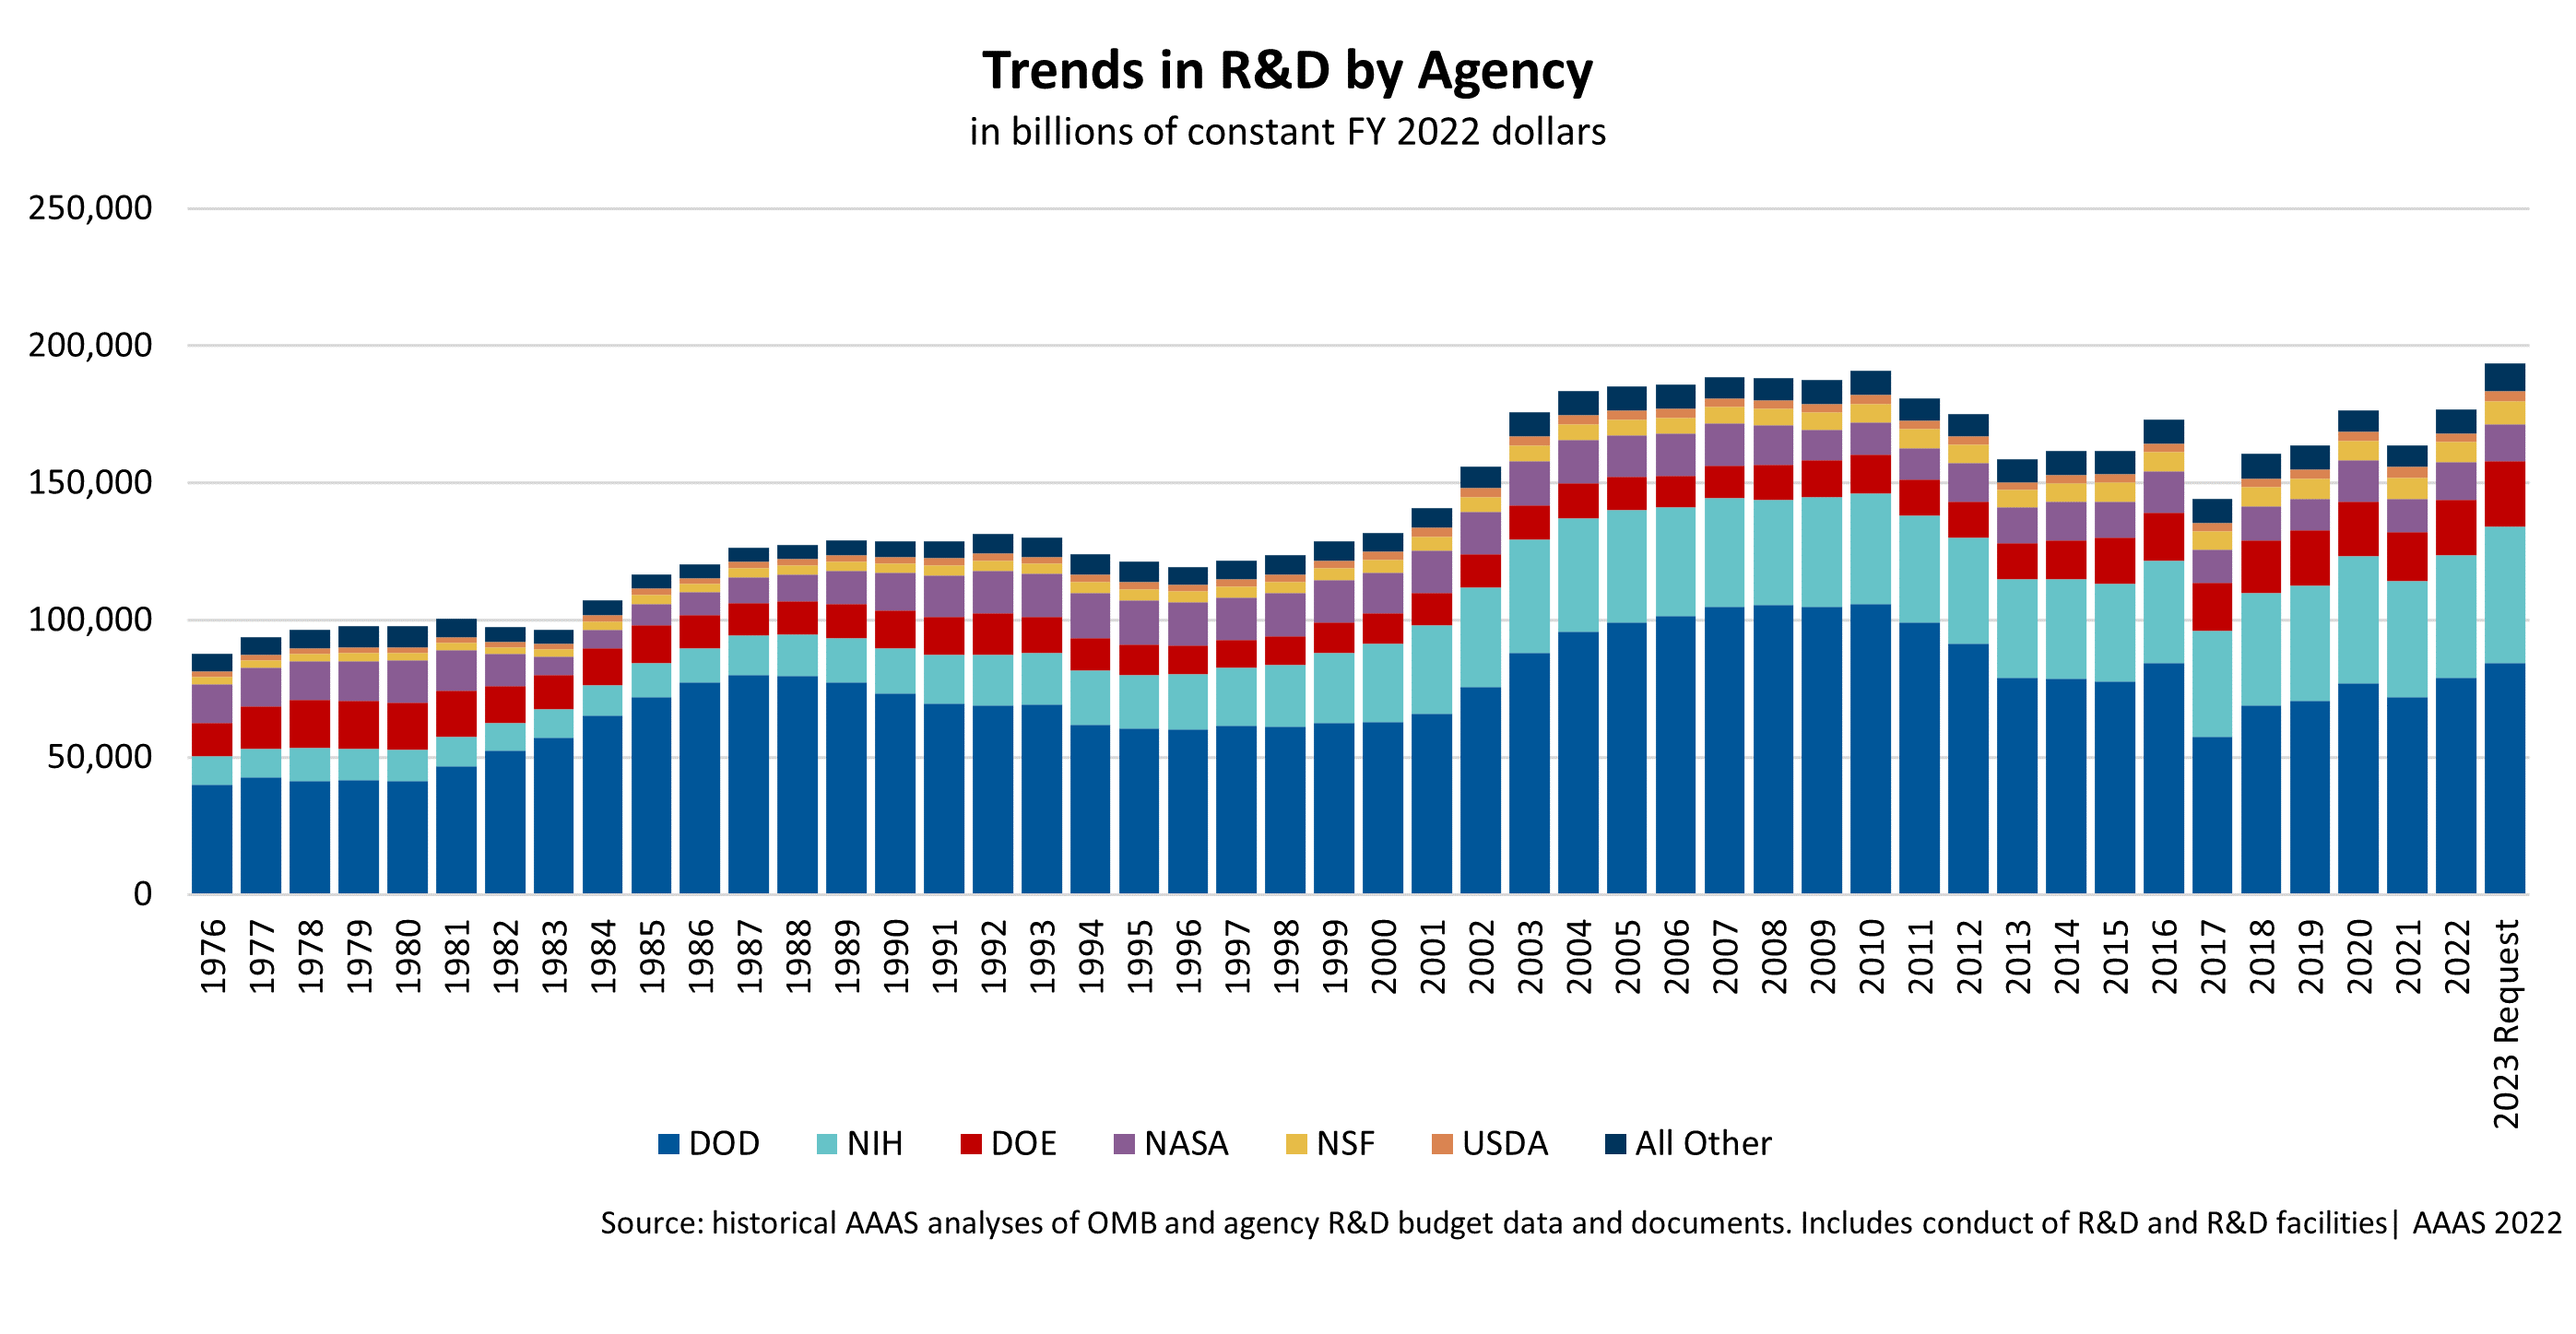
\includegraphics[width=\textwidth]{Agencies.png}
%\end{center}
%}
%\only<2>{
% \begin{center}
% 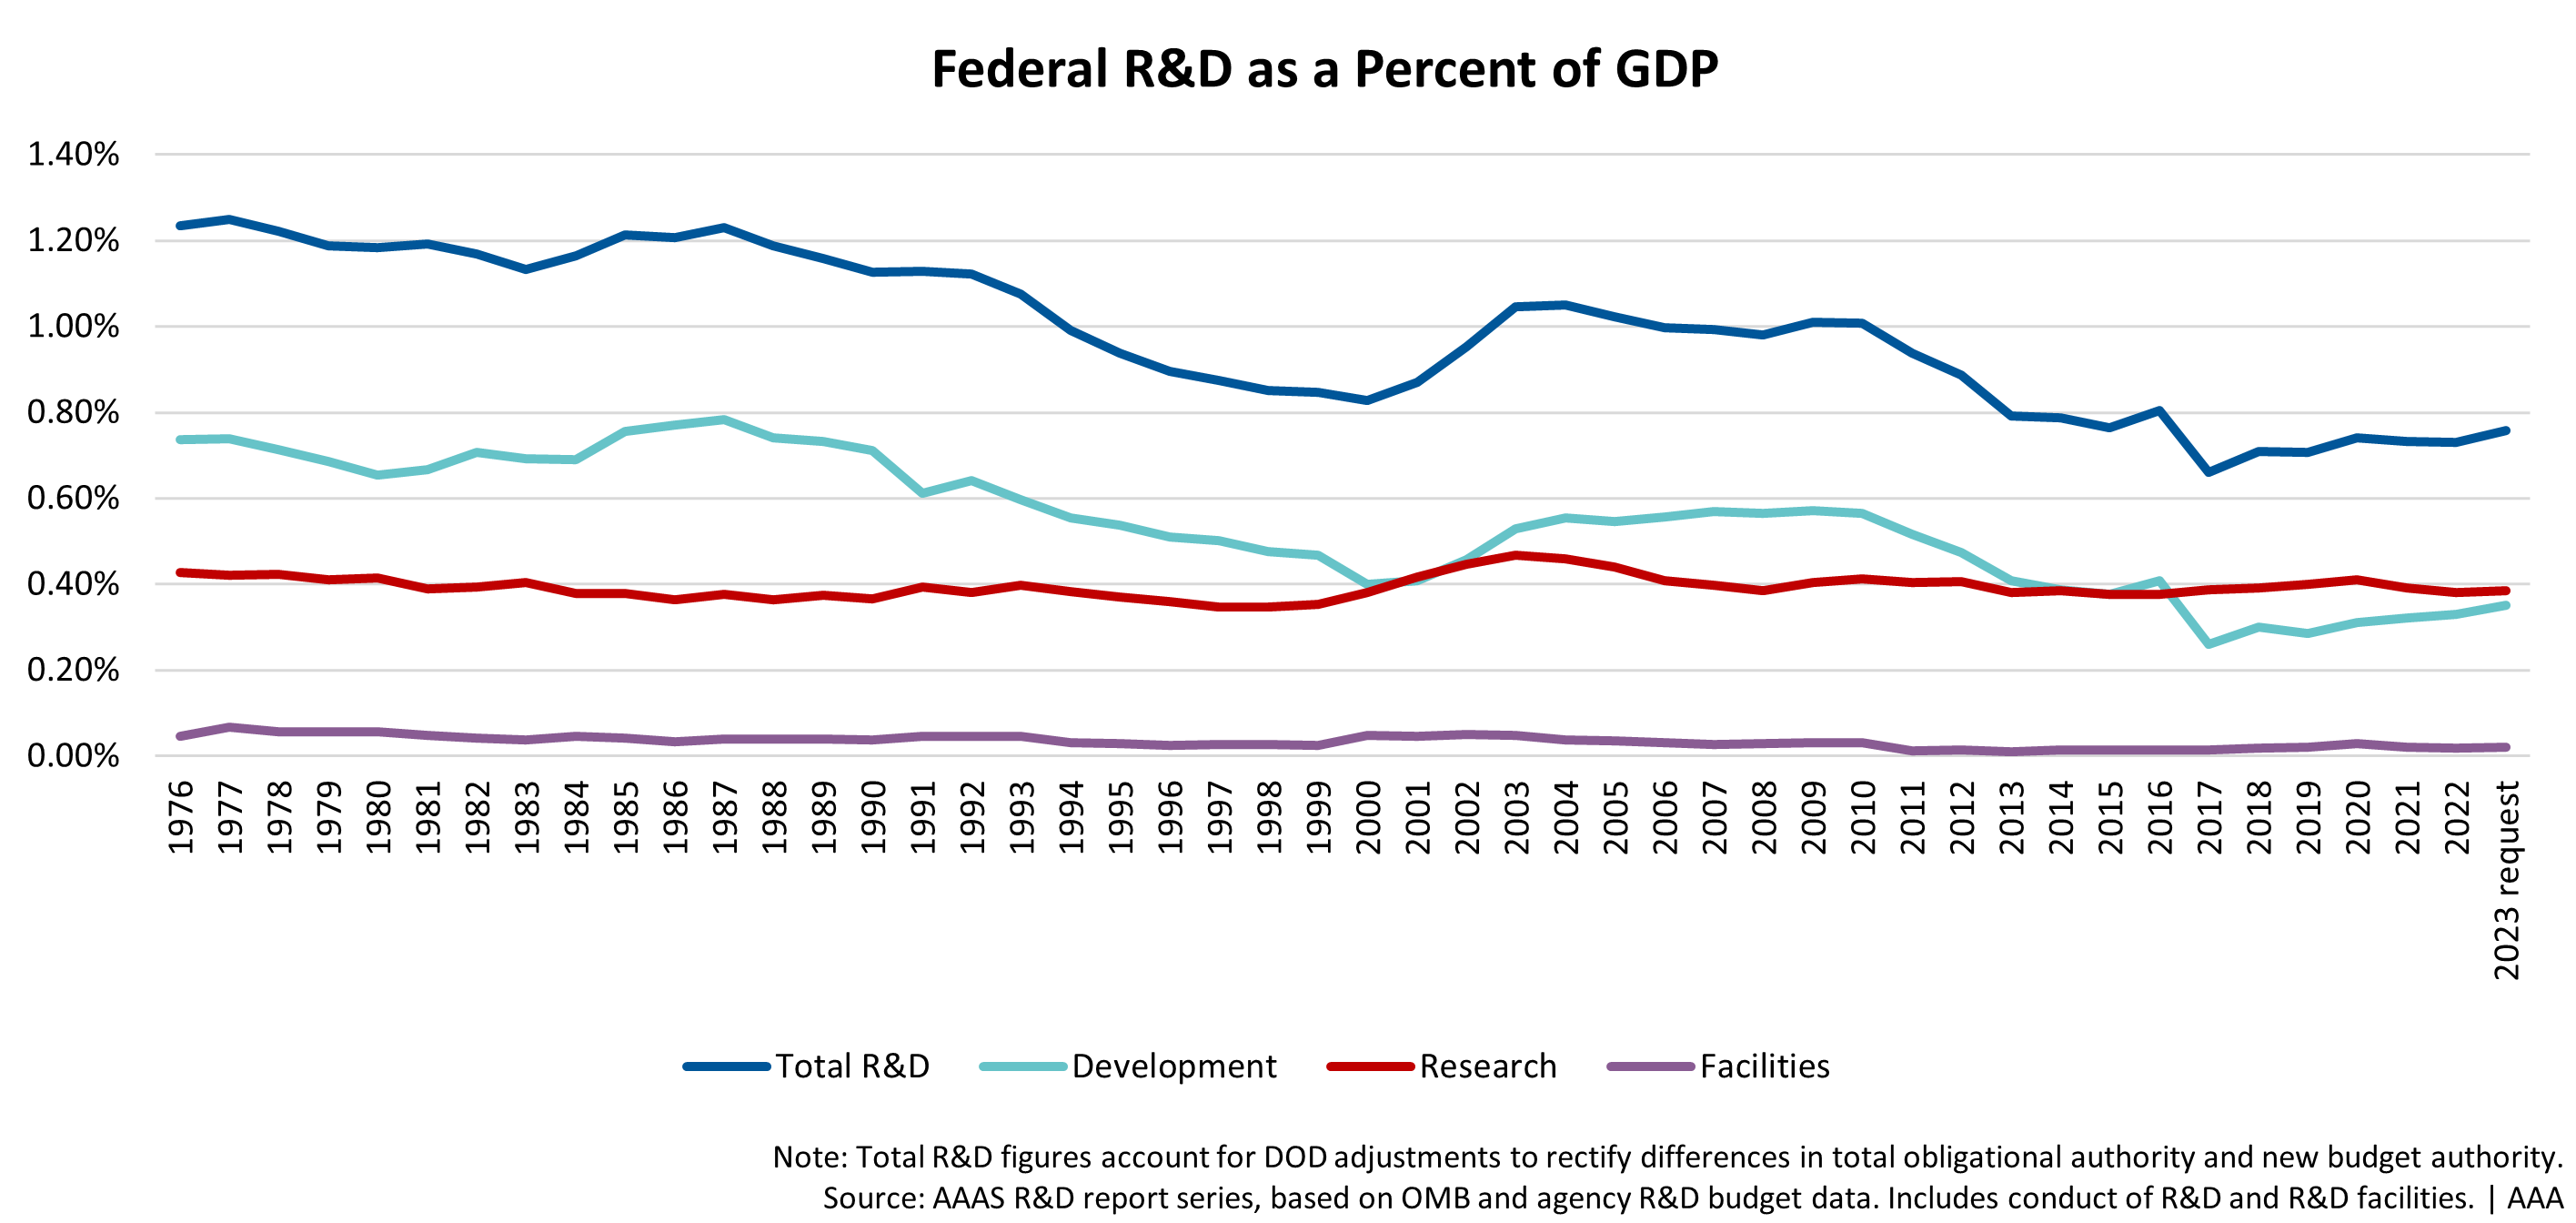
\includegraphics[width=\textwidth]{RDGDP.png}
%\end{center}
%}
%%\only<4>{
%% \begin{center}
%% 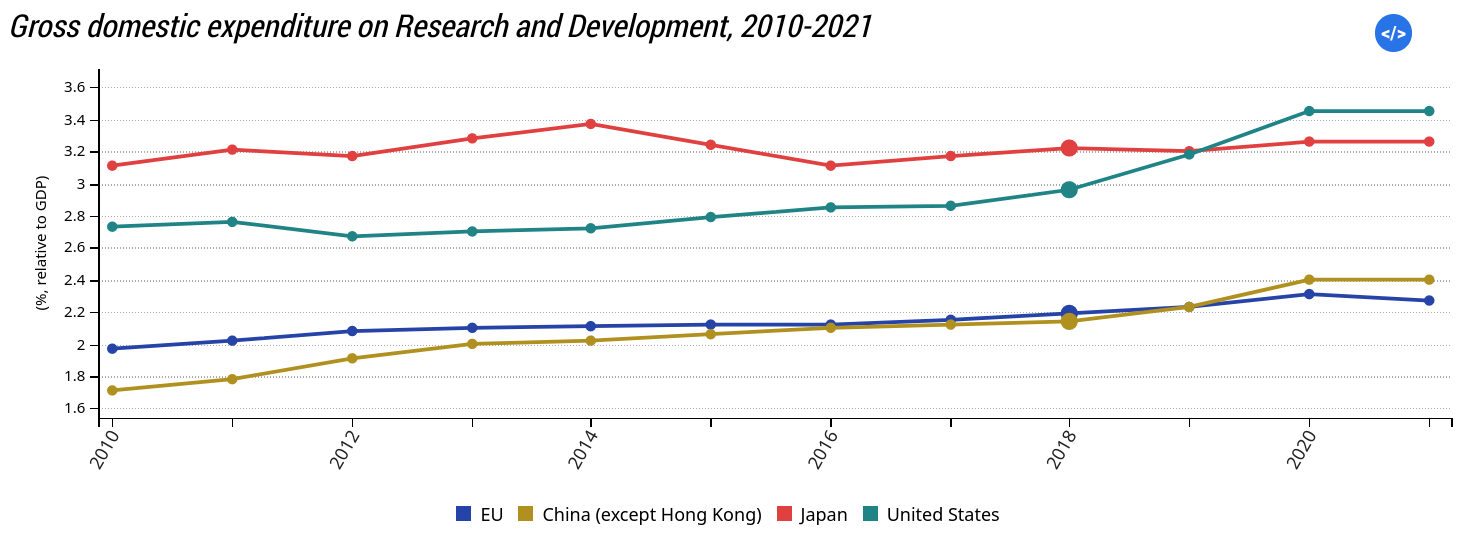
\includegraphics[width=\textwidth]{RDGDP-global.png}
%%\end{center}
%%}
%\end{frame}
%
% %%%
%
%\subsection{Symbiotic relation between Publishers and Universities}
%
% \begin{frame}[t]{New scientific publishing mechanisms}
%\begin{itemize}
%
% \item 1951: Pergamon Press (now \textbf{Elsevier}) and R. Maxwell: many new thematic journals
%   %1951: Robert Maxwell creates Pergamon Press. Academic journals used to be mainly owned by learned societies. Maxwell perceives the potential huge profitability of academic publishing as the public funding for research rises. He creates many new journals for specific fields of research and surfs on globalisation with grand titles like ‘International Journal of’. Pergamon Press is sold to Elsevier in 1991. [13]
% \item 1955: appearance of \textbf{impact factor}
%   % The idea of an impact factor is first mentioned by Eugene Garfield in Science. It was originally thought of as a tool for librarians to identify journals to purchase, not as a measure of the quality of research [14]. Since 1975, it has been computed and published in the Journal Citation Reports (JCR), nowadays owned by Clarivate [15].
% \item 1970s: rise of journals subscriptions $\Rightarrow$ emerging crisis
%   % Beginning of the serials pricing crisis: the prices of subscriptions to scholarly journals rise tremendously. For instance, between 1973 and 1987, the average price increases by 12\% per year, while the costs for the publishers only rise increase by 8\% [16, p. 22]. This difference between expenses and revenue enables the publishers to make big margins. Librarians start to organise and fight back.
% \item 1991: creation free archive \textit{xxx.lanl.gov} at Los Alamos National Laboratory (to become \textbf{arXiv.org}).
%% Paul Ginsparg creates the free archive xxx.lanl.gov at Los Alamos National Laboratory, which will become arXiv.org 10 years later [17].
%\item By 1994, three years after acquiring Pergamon, Elsevier had raised its prices by 50\%. Librarians began cancelling subscriptions to less popular journals.
%\end{itemize}
%
%\fig{.35}{Open_Access_PhD_Comics}
%\hspace{1cm}
%\fig{.3}{price_increase_publisher_phd_comics}\\
%  \begin{center}
%    \small
%    Graphic from \href{http://www.phdcomics.com/comics.php?f=1533}{PHD Comics}
%  \end{center}
%\end{frame}
%
% %%%
%
%\begin{frame}[t]{What is the problem?}
%  \fig{.6}{cash_flow}
%\end{frame}
%
%%%%
%
% \subsection{Advent of Open Access}
%
% \begin{frame}[t]
%  \begin{center}
%  \vspace{3cm}
%  {\huge Open Access}\\
%  \end{center}
%\end{frame}
%
%%%%% 
%
% \begin{frame}[t]{Advent of open access}
%\begin{itemize}
%
%\item 2000: Foundation of \textbf{BioMed Central} publisher (now in Springer Nature) and online open-access with \textbf{article processing charge (APC)}
% % Foundation of \textit{BioMed Central} publisher and by Vitek Tracz. This publisher inaugurates a business model based on online open-access journals with an article processing charge (APC). It is now part of Springer Nature. [18]
%\item 2000: 34,000 scientists petition:
%  \begin{quote}
%    “we will publish in, edit and review for, and personally subscribe to only those scholarly and scientific journals that have agreed to grant unrestricted free distribution rights to any and all original research reports.”
%  \end{quote}
%  Leads to \textbf{the Public Library of Science (PLoS)}, with APC
%
%  \item 2002: \textbf{Budapest Open Access Initiative (BOAI)}: promotes open access \textbf{but} no recommendation for the costs
%    %Budapest Open Access Initiative (BOAI). This landmark conference on the open access movement is organised by the Open Society Institute. It results in a public call to promote open access of scholarly literature, insisting on the need to remove all access fees for the readers, but it does not promote any particular model to cover the costs. [20]
%  \item 2005: The Wellcome Trust foundation: \textbf{funding requires output open access}
%    % The Wellcome Trust, a British research foundation, starts requiring open access for the research they fund. [21]
%  \item 2018: \href{https://www.snf.ch/en/bQ17hb9mM1NC4awy/news/news-181010-make-open-access-the-new-normal}{SNF allows to budget OA APC}
%  \item 2021: \href{https://www.coalition-s.org/}{The Plan/cOAlition S}: requires Open Access journals or platforms. Followed by \href{https://www.coalition-s.org/supporters/}{many institutions}
%    %requires scientific publications resulting from research funded by public grants to be published in compliant Open Access journals or platforms. It is supported by major institutions such as the World Health Organization, the Bill \& Melinda Gates Foundation, the European Commission. [23]
% \end{itemize}
%\end{frame}
%
%%%% 
%
%
%\section{Open Access}
%\subsection{Open Access models}
%
%\begin{frame}[t]{No more problem?}
%\fig{.6}{cash_flow_GOA}
%\end{frame}
%
%%%%
%
%\section{Publication Costs}
%\subsection{Rigorous publication costs estimation}
%\begin{frame}[t]{Cost of a publication?}
%
%\href{https://doi.org/10.12688/f1000research.27468.2}{Grossmann, A. \& Brembs, B. Current market rates for scholarly publishing services. (2021)} 
%\begin{quote}
%  \vspace{.5cm}
%   [...] conservative estimates show that the publication cost for a representative scholarly article \textbf{is around \$400}.
% \end{quote}
%
% \pause
% \vfill
%\centering{
% \Large{How to evaluate such a cost?}}
%\end{frame}
%
%%%%
%
%\begin{frame}[t]{Editorial cost of a publication?}
%\begin{quote}
%  \vspace{-.2cm}
%   [...] conservative estimates show that the publication cost for a representative scholarly article \textbf{is around \$400}.
% \end{quote}
%
%  \begin{minipage}{.45\textwidth}
%   \textbf{Content acquisition}
%   \begin{itemize}
%   \item Authors (re-)submission
%   \item Dealing with reviewers
%   \item Plagiarism/Similarity check
%   \item DOI for paper\&reviews
%   \item APC collection
%   \end{itemize}
% \end{minipage}
% \hfill
%   \pause
% \begin{minipage}{.45\textwidth}
%   \textbf{Content preparation}
%   \begin{itemize}
%   \item Manuscript tracking
%   \item Production check-in
%   \item Manuscript Technical checking
%   \item Copyediting, Typesetting, Figures/graphs/tables
%   \item Metadata, metrics
%   \item Authors corrections
%   \end{itemize}
%\end{minipage}
%\vfill
%\pause
%\begin{center}
% \begin{minipage}{.7\textwidth}
%  \textbf{Dissemination/archiving}
%  \begin{itemize}
%  \item Web OA platform and hosting
%  \item Long-term digital preservation
%  \item Distribution to indexing services (Scopus, PMC, DOAJ, ...)
%  \end{itemize}
%\end{minipage}
%\end{center}
%\end{frame}
%
%
%%%%
%
% \subsection{Article Processing Charges}
%\begin{frame}[t]{Cost of APCs?}
%
%  \begin{quote}
%   [...] conservative estimates show that the publication cost for a representative scholarly article \alert{is around \$400}.
% \end{quote}
% \pause
%
% \begin{center}
% \alert{\Large Yet APCs scale with impact factor}\\
% \end{center}
%
% \pause
% \fig{.6}{publisher-APC}
%
%\end{frame}
%
%%%%
%
%\subsection{Publisher Revenues}
%\begin{frame}[t]{Publisher revenues}
% \fig{.5}{publishers-revenues}
% \begin{quote}
%   Revenues in 2020 of the biggest publishers in \$
%
%   \href{https://doi.org/10.5281/zenodo.7212922}{Against Parasite Publishers: Making Journals Free (2022)}
%
% \end{quote}
%\end{frame}
%
%%%%%
%\subsection{Publisher Margins}
%\begin{frame}[t]{Publisher margins}
% \fig{.55}{publisher-margins}
% \begin{quote}
%
%   Declared Operating margins in 2020 in \%
%
%   \href{https://doi.org/10.5281/zenodo.7212922}{Against Parasite Publishers: Making Journals Free (2022)}
%
%
%\end{quote}
%\end{frame}
%
%%%% 
%
%\begin{frame}[t]{Open Access Models}
%
%\href{ https://oabooks-toolkit.org/lifecycle/article/13868103-green-gold-diamond-different-models-for-open-access-books}{Credits to oabooks-toolkit}
%  \vfill
%
% 
% \begin{itemize}
% \item Gold
%   \begin{itemize}
%   \item Immediate open access publication
%   \item Managed by the publisher (\textbf{APCs})
%   \item \textbf{licence allowing reuse (e.g. Creative Commons)}
%   \end{itemize}
%   \pause
% \item Green (self-archiving)
%   \begin{itemize}
%   \item Publication archived online in an \textbf{Open-access repository} (arXiv, HAL, infoscience).
%   \item \textbf{No publisher work} (copy-editing, proofreading, typesetting, indexing, metadata tagging, marketing or distribution).
%   \item Not listed by publishers (\textbf{no metrics})
%   \end{itemize}
%\pause
% \item \textbf{Diamond}\newline
% \begin{quote}
%   \textbf{Diamond open access} refers to academic texts (such as monographs, edited collections, and journal articles) published/distributed/preserved with \textbf{no fees to either reader or author.} 
% \end{quote}
%\pause
%\item \textbf{Overlay journal}\newline
% \begin{quote}
%   An \textbf{open access} academic \textbf{overlay journal} does not produce its own content, but selects from texts that are \textbf{already freely available online}.
% \end{quote}
%
% \end{itemize}
%
%\end{frame} 
%%%%
%
%\subsection{SNF Open Access recommendations}
%\begin{frame}[t]{SNF Open access recommendations}
%
%  \begin{center}
%    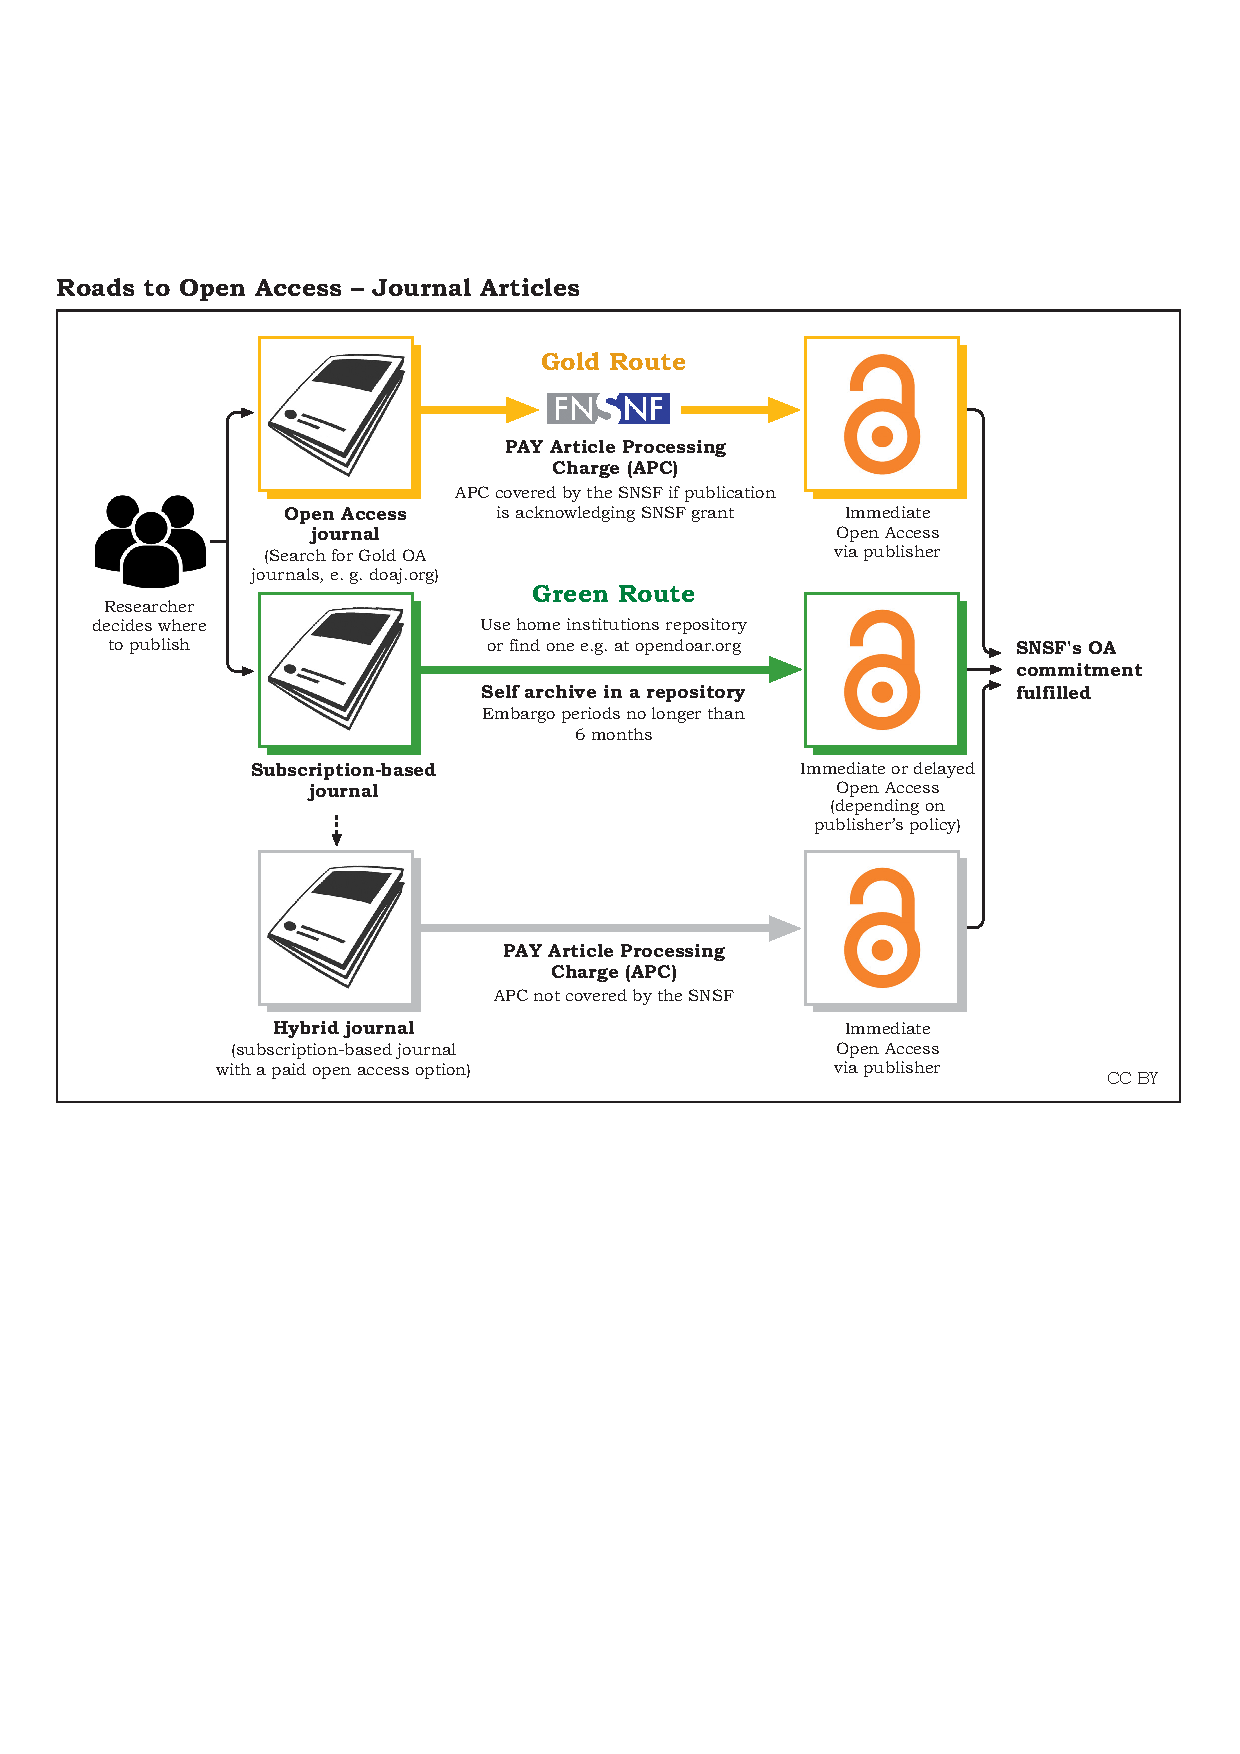
\includegraphics[width=.65\textwidth]{SNSF_Roads_to_OA_Articles}
%  \end{center}
%  \href{https://www.snf.ch/en/VyUvGzptStOEpUoC/topic/open-access-to-publications}{Illustration from www.snf.ch}
%\end{frame}
%
%
%%%%
%
%%\begin{frame}[t]
%%  \begin{center}
%%  \vspace{3cm}
%%  {\huge Diamond Open Access}\\
%%  \end{center}
%%\end{frame}
%%
%%%%
%%\section{Diamond Open Access}
%%\subsection{DOA definitions and figures}
%%\begin{frame}[t]{Diamond Open Access}
%%
%%Wikipedia Definition:\newline \newline
%% \begin{quote}
%%   \textbf{Diamond open access} refers to academic texts (such as monographs, edited collections, and journal articles) published/distributed/preserved with \textbf{no fees to either reader or author.} \newline
%% \end{quote}
%% \pause
%%\href{https://doi.org/10.5281/zenodo.4558704}{OA Diamond Journals Study. Part 1: Findings. (2021)\newline}
%%
%%\textbf{Landscape}\\
%%\begin{itemize}
%%\item $\sim 29000$ DOA journals (30\% in DOAJ)
%%\item Fewer articles (356000 per year vs. 453000 APC ones), average $\sim$ 25 articles/year
%%\item Since 2018 $\searrow$ DOA articles while $\nearrow$ of APC-ones
%%\item 45\% in Europe, 25\% in Latin America, 16\% in Asia, \textbf{5\% in the US/Canada}
%%\item 60\% HSS, 22\% science, 17\% medicine
%%\end{itemize}
%%
%%\end{frame}
%%
%%%%%
%%
%%\begin{frame}[t]%
%% \titleframe{Diamond Open Access}\vskip1cm%
%%
%%Wikipedia Definition:\newline \newline
%% \begin{quote}
%%   \textbf{Diamond open access} refers to academic texts (such as monographs, edited collections, and journal articles) published/distributed/preserved with \textbf{no fees to either reader or author.} \newline
%% \end{quote}
%%
%%\href{https://doi.org/10.5281/zenodo.4558704}{OA Diamond Journals Study. Part 1: Findings. (2021)\newline}
%%
%%\textbf{Sustainability and funding}\\
%%\begin{itemize}
%%  \item 60\% of DOA journals depend on volunteers
%%  \item The majority (53\%) run with less than 1 FTE
%%  \item 70\% declared less than \$/€10,000 annual costs.
%%  \item Funding mainly by Universities, and much less by Funding agencies
%%\end{itemize}
%%\end{frame}
%%
%%%%%
%%
%%\subsection{DOA in Switzerland}
%%
%%\begin{frame}[t]%
%% \titleframe{Diamond open in CH}\vskip1cm%
%%
%%{\small
%% \href{https://zenodo.org/doi/10.5281/zenodo.7461727}{Mapping the Swiss Landscape of Diamond Open Access Journals. The PLATO Study on Scholar-Led Publishing. Report}\\
%% \href{https://www.unige.ch/biblio/fr/actus/projet-plato/}{Projet PLATO: l’Open Access Diamant est en bonne voie en Suisse - Bibliothèque - UNIGE (2023)}
%%}
%% \vfill
%%
%%\begin{minipage}{.49\textwidth}
%%   \textbf{Key Findings}
%%   \begin{itemize}
%%   \item 186 journals (very diverse)
%%   \item $< 25$ articles/year, mostly peer reviewed
%%   \item Motivation: visibility, OA policies
%%   \item Proofreading: \textbf{well above average}
%%   \item Editorial tasks: (young) volounteers
%%   \item Sustainability (fundraising) is a challenge
%%   \item Costs: \textbf{average CHF 433/article} 
%%   \end{itemize}
%% \end{minipage}
%% \begin{minipage}{.49\textwidth}
%%\pause
%%   \textbf{Key Learnings}
%%   \begin{itemize}
%%   \item Driving force: \textbf{opening practices}
%%   \item High Quality $\neq$ equity sacrifice
%%   \item Needs funding to
%%     \begin{itemize}
%%     \item pay collaborators and improve quality
%%     \item outsource services (design, IT, typesetting)
%%     \item give recognition 
%%     \item achieve \textbf{long-term stability}
%%     \end{itemize}
%%   \end{itemize}
%%
%% \end{minipage}
%% \vfill
%% \pause
%% \begin{quote}
%%   The term \textit{Diamond OA} is intricately linked to \textbf{a not-for-profit business model} based on \textbf{institutional funding} and \textbf{ownership} by the research community, on \textbf{collaborative work} between researchers having shared values of \textbf{equity and diversity}
%% \end{quote}
%%
%%\end{frame}
%
%%%% 
%
%
%\section{JTCAM}
%
%\subsection{JTCAM description}
%\begin{frame}[t]
%  \begin{center}
%  \vspace{1cm}
%  \fig{.8}{logo2023}\\
%  \vspace{.2cm}
%  \textit{Diamond Open Access, Overlay journal}\\
%  \end{center}
%  \fig{.6}{equipe2_}
%  
%\end{frame}
%
%%%%
%
%\begin{frame}[t]
%  \fig{.6}{logo2023}
%  \begin{itemize}
%  \pause  \item \textbf{Overlay Journal}
%   \begin{itemize}
%   \item Always a preprint shared on Open Archives (even for refused papers)
%   \item Diamond Open Access
%   \item FAIR open access (\textbf{F}indable, \textbf{A}ccessible, \textbf{I}nteroperable, \textbf{R}eusable)
%   \end{itemize}
%   \pause
% \item \textbf{Team}
%   \begin{itemize}
%   \item Technical board: creators of the journal + data/software editor
%   \item Scientific Board: invited
%   \item Editorial board: elected
%   \item Collegial decisions
%   \end{itemize}
%   \pause  
% \item\textbf{Peer Reviewed}
%   \begin{itemize}
%   \item Publish reviewers' work as Open Reviews
%   \end{itemize}
%   \pause
% \item\textbf{Data\&Software Review/Curation}
%   \begin{itemize}
%   \item Strong incentive for \textbf{reproducibility} (ongoing)
%   \end{itemize}
%   \pause
% \item \textbf{Copy-editing}
%   \begin{itemize}
%   \item Very high quality
%   \end{itemize}
% \end{itemize}
%\end{frame}
%
%
%%%%
%
%
%%\subsection{Community}

%
%\subsection{FAIR principles addressed}
%\begin{frame}[t]{JTCAM FAIR principles}
%  \textbf{F}indable by Journal indexation
%  \begin{itemize}
%  \item \textit{Directory of Open Access Journals} (\href{https://doaj.org/}{DOAJ}), \textit{Free Journal Network} (\href{https://freejournals.org/}{FJN}), \textit{International Standard Serial Number International Center} (\href{https://www.issn.org/}{ISSN}), \href{https://reseau-mirabel.info/}{Mir@bel}
%  \end{itemize}
%\vfill
%  \textbf{A}ccessible
%  \begin{itemize}
%  \item OpenSource \href{https://www.episciences.org/}{Episcience} CMS (funded by French \href{https://www.ccsd.cnrs.fr/}{CCSD} through CNRS, INRIA, INRAE, OpenAIRE, FNSO)  
%  \item Overlay Journal: articles stored in open repositories (\href{https://arxiv.org/}{arXiv}, \href{https://hal.science/}{HAL})
%  \item Curated/Reviewed Datasets with DOI \href{https://zenodo.org/}{@Zenodo} (Curation with ETH-ORD)
%  \item \href{https://creativecommons.org/share-your-work/cclicenses/}{CC-BY license} 
%  \end{itemize}
%  \vfill
%  \textbf{I}nteroperable
%  \begin{itemize}
%  \item Provided by the repositories with metadata
%  \end{itemize}
%\vfill
%  \textbf{R}eusable
%  \begin{itemize}
%  \item Saving Software revision \href{https://www.softwareheritage.org/}{@Software Heritage} (SWHID $\sim$ DOI for software) complement datasets  
%  \end{itemize}
% 
%\end{frame}
%
%
%\begin{frame}[t]{JTCAM: Challenges}
%  \begin{itemize}
%  \item 37 articles published (15 refused, 70\% acceptance)
%    \begin{itemize}
%    \item Mostly from French community (90\%)
%    \item Difficult to become international
%    \end{itemize}
%  \item Copy-editing
%    \begin{itemize}
%    \item Low motivation on authors' side
%    \item Lots of work for technical editors (> 10h of work per paper)
%    \item Fairly long time between acceptation and publication (4 months acceptance + 2 months copy-editing with datasets review) 
%    \end{itemize}
%  \item Open Data/Open Software 
%    \begin{itemize}
%    \item Cultural limitations (for mechanics)
%    \item Development of curation tool (ETH-ORD funding)
%    \end{itemize}
%  \end{itemize}
%\vfill
%\pause
%  \textbf{JTCAM bets on:}
%\begin{itemize}
%  \item Open ethical principles
%  \item Overlay model (thanks to \href{https://www.episciences.org/}{Episciences})
%  \item Review+copy editing quality (paper+datasets)
%\end{itemize}
%  
%\end{frame}
%
%%%%
%%\subsection{Problematic of science metrics}
%%\begin{frame}[t]{Community adhesion challenge}
%%
%%  \textbf{Lack of journal metrics is fearsome for JTCAM authors}
%%  \begin{itemize}
%%  \item Authors fear for impact (for young investigators carreers)
%%  \item Reputation takes time to build
%%  \item Imbalance between countries incentives (rich vs. poorer countries)
%%  \end{itemize}
%%
%%  \vfill
%%  
%%  \textbf{San Francisco Declaration on Research Assessment (DORA, 2013)}
%%  \begin{quote}Do not use journal-based metrics, such as Journal Impact Factors, as a surrogate measure of the quality of individual research articles, to assess an individual scientist’s contributions, or in hiring, promotion, or funding decisions.\end{quote}
%%
%%  \textbf{Coalition for Advancing Research Assessment (CoARA, )}
%%\begin{quote}
%%The Agreement on Reforming Research Assessment sets a shared direction for changes in assessment practices for research, researchers and research performing organisations, with the overarching goal to maximise the quality and impact of research.
%%\end{quote}
%%  \vfill
%%    
%%\end{frame}
%%%%
%
%
%\section{Open Data}
%%%%
%
%\begin{frame}[t]
%  \begin{center}
%  \vspace{3cm}
%  {\huge Open Data}\\
%  \end{center}
%\end{frame}
%
%%%%
%
%\subsection{Data cycle}
%\begin{frame}[t]{Data cycle: \href{https://ethrat.ch/wp-content/uploads/2023/06/ETH-ORD-Report_version3.pdf}{ETH Domain report}}
%  \fig{.8}{data-workflow}
%\end{frame}
%
%%%%
%
%\begin{frame}[t]{On fait le point sur les données...}  
%\begin{center}
%  \url{https://zenodo.org/records/10108736}\\
%\end{center}
%  \fig{.6}{data-cycle}
%\end{frame}
%
%
%%%%
%
%\subsection{What makes datasets useful ?}
%\begin{frame}[t]{What makes (open) datasets useful: FAIR}
%
%  \textbf{F}indable
%  \begin{itemize}
%    \item Need for searchable databases
%    \item Annotation (keywords, cross-links, ownership, ...)
%    \item \textit{Digital Object Identifier} (DOI)
%  \end{itemize}
%\vfill
%  \textbf{A}ccessible
%  \begin{itemize}
%    \item Retention times
%    \item Choice of data repository
%    \item Question of storage costs   
%  \end{itemize}
%  \vfill
%  \textbf{I}nteroperable
%  \begin{itemize}
%  \item Compatibility issues (beetween repositories, packages, file formats, ...)
%  \end{itemize}
%\vfill
%  \textbf{R}eusable
%  \begin{itemize}
%    \item Operating context (Software versions, dependencies, ...)
%    \item Open (source) licences
%  \end{itemize}
%
%\end{frame}
%
%%%%
%
%
%\begin{frame}{Need for annotation and cleaning}
%\fig{.45}{comics3}\\
%\begin{center}
%  \url{https://zenodo.org/records/10108736}
%  \end{center}
%\end{frame}
%
%%%%
%
%\subsection{Journals policies with datasets}
%\begin{frame}{Journals policies with datasets}
%
%
%e.g. the \href{https://www.springernature.com/gp/authors/research-data-policy}{Springer research data policy}\newline
%
%\href{https://group.springernature.com/gp/group/media/press-releases/archive-2016/over-600-springer-nature-journals-commit-to-new-data-sharing-policies/12000254}{Classification of journals}
%\begin{tabular}{ll}
% Type 1 & Data sharing and data citation is encouraged                            \\
% Type 2 & Data sharing and evidence of data sharing encouraged                    \\
% Type 3 & Data sharing encouraged and statements of data availability required    \\
% Type 4 & Data sharing, evidence of data sharing and peer review of data required \\
%\end{tabular}\newline\newline
%\pause
%$\Rightarrow$ \textbf{(Computational) mechanics should be of type 4}
%\pause
%\vfill
%
%\begin{itemize}
%  \item Springer journals created for reviewing datasets (\href{https://www.springernature.com/gp/authors/research-data/research-data-publishing}{Scientific Data, BMC series, Discover})
%  \item The \href{https://joss.theoj.org/about}{Journal of Open Source Software (JOSS)}, Open Source Initiative\\
%\pause
%  \item and now \href{https://jtcam.episciences.org/}{JTCAM} $\Rightarrow$ ambitious goals
%\end{itemize}
%\pause
%\vfill
%\begin{center}
%{\Large Makes sense to gather the review of paper and datasets}
%\end{center}
%\end{frame}
%
%%%%
%

%%%
